\section{Design}
\label{sec:design}
\textit{Her kommer detaljene om \textbf{hvordan} en har tenkt at konseptet skal kunne fungere. Det er fremdeles snakk om prinsipper og ideer, ikke fysisk realisering og komponentvalg.}

\subsection{Systemets sammenheng}

Systemets informasjonsflyt er illustrert i figur \ref{fig:blokkDig}. Her skal det infrarøde kameraet sende video kontinuerlig til prosesseringsenheten som skal detektere om en det er en/flere fugl(er) i bildet. Samtidig skal prosesseringsenheten ta inn data fra værsensorene og tolke disse. Disse dataene sende så videre til en database. En nettside skal så hente vise fram dataen fra databasen, slik at brukeren får et oversiktlig bilde over fugleaktiviteten i området. 

\begin{figure}[H]
    \centering
    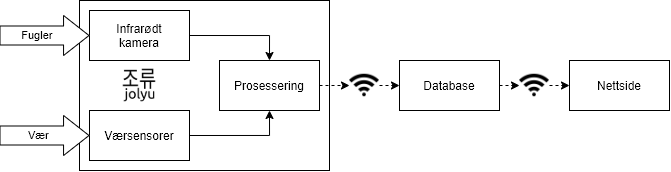
\includegraphics[width=0.9\textwidth]{konsept/diagram_konsept_v4.png}
    \caption{Blokkdiagram for hvordan produktet skal fungere. Fuglene blir detektert av et infrarødt kamera og bildene prosesseres. Dataen blir så sendt videre til en database og vist fram på en nettside.}
    \label{fig:blokkDig}
\end{figure}


\subsection{Kamera}

Et infrarødt kamera (IR-kamera) brukes til å detektere infrarød stråling fra objekter. Infrarød stråling er elektromagnetisk stråling, slik som synlig lys, med en bølgelengde mellom 7$\mu$m og 1mm\cite{SNL-IR}. Dette gjør at et IR-kamera kan se forskjellen i temperatur til objekter.
\todo{Kilde?}
Sensorer i dette spekteret kan detektere alle objekter med en temperatur over det absolutte nullpunkt, 0K (-273.15$\degree$C), og opp til 3864K (4137$\degree$C). I vårt tilfelle vil IR-kameraet bruke temperaturen til omgivelsene og legemet vi skal observere, samt forventet emissiviteten for observasjonelegemt. Kroppstemperaturen til fugler ligger ved omtrent 40$\degree$C \cite{fugltemp}, og omgivelsene kan antas å holde mellom -15$\degree$C og 30$\degree$C utifra maks og minimum temperatur i Trondheim. Emissiviteten til fugler er målt til å være ca. 0.95 \cite{fuglemm}.


\todo{Kameraet vet vel ikke $\epsilon$ til objektet. Brukes $\epsilon=1$?}
Et IR-kamera bruker Stefan-Boltzmanns lov for å regne ut temperaturen til objektet: $\Theta=\epsilon \sigma T^4$, der $\Theta$ er varmestrålingseffekt per areal (W/$m^2$), T er temperatur i kelvin, $\sigma$ er Boltzmanns konstant og $\epsilon$ er den termiske emissiviteten til objektet som skal måles. For fugler er denne emissiviteten målt til å være ca. 0.95 \cite{fuglemm}.

\todo{Kanskje legge til emmisiviteten til himmelen}

\subsection{Deteksjon}

Prosesseringsenhetesn skal få inn en kontinuerlig strøm av bilder fra kameraet og behandle denne bilde for bilde. Bildebehandlingen skal finne objekter i bildet, eller såkalte ''blobs''. Objektene som skal oppdages er fugler, og disse vil skille seg ut fra bakgrunnen på grunn av deres høyere temperatur, som representeres ved at de har ulik farge fra bakgrunnen. Bildebehandlingen skal kunne detektere flere objekter i samme bilde. I tillegg skal den kunne se på forrige bilde
for å finne ut om en blob har beveget seg, og dermed kunne følge denne bloben gjennom en bildeserie. Slik unngås det at hver fugl telles en gang per bilde, men blir i stedet fulgt fra den kommer inn i synsbredden til kameraet til den går ut, og teller det som én fugl.

I utgangspunktet skal systemet detektere fugler i et område foran vindturbinen der det vil være stor fare for at om fuglen detekteres så vil den kollidere med vindturbinen. Deteksjonsområdet vil dekke minst området som er vist i figur \ref{fig:TurbinForan} og i figur \ref{fig:TurbinSiden}. I 3 dimensjoner vil dette se ut som en invertert pyramide. Grunnen til at deteksjonsområdet sett fra siden ikke er flat ($\beta \approx 0$) er for at vi skal kunne detektere retningen til fuglen for å kunne konkludere at den treffer vindturbinen eller ikke. I tillegg er det ikke gunstig om vindturbinen er i deteksjonsområdet da dette vil kunne skape interferens med målingene våre. 


\begin{figure}[H]%hentet fra https://www.cadblocksfree.com/en/wind-turbine.html
  \centering
  \begin{minipage}[b]{0.45\textwidth}
    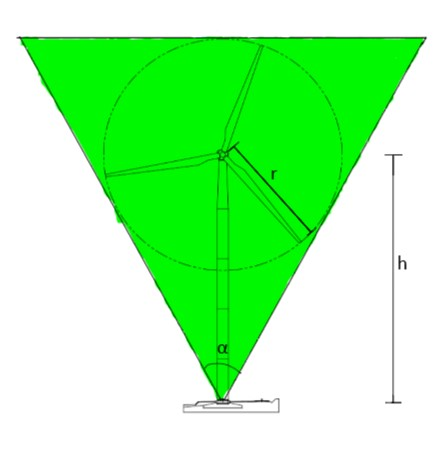
\includegraphics[width=\textwidth]{design/DeteksjonForan.jpg}
    \caption{Deteksjonsområdet til systemet sett fra framsiden til vindturbinen, markert i grønt. }
    \label{fig:TurbinForan}
  \end{minipage}
  \hfill
  \begin{minipage}[b]{0.45\textwidth}
    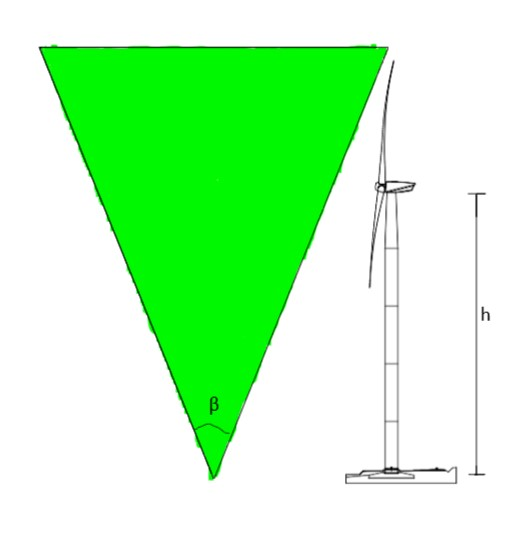
\includegraphics[width=\textwidth]{design/DeteksjonSiden.jpg}
    \caption{Deteksjonsområdet til systemet sett fra siden til vindturbinen, markert i grønt.}
    \label{fig:TurbinSiden}
  \end{minipage}
\end{figure}



\subsection{Værstasjon}
Systemet skal ha egne sensorer for innsamling av værdata. Dette vil være sensorer for måling av lufttrykk, lufttemperatur, luftfuktighet, vindstyrke, vindretning og regn. Dataene fra sensorene skal deretter knyttes opp mot fugleaktiviteten for å finne eventuelle sammenhenger i vær og fugleaktivitet. For eksempel, hvis all fugleaktivitet skjer når det ikke blåser, så vil kollisjon med vindturbiner være en mindre reell fare, da turbinene ikke beveger seg i slikt vær. 

\subsection{Strukturelt}

Prosesseringsenheten og kameraet skal dele en boks. Boksen skal være over bakkenivå for å unngå forstyrrelser fra dyr nære bakken, og for å ikke tildekkes av snø eller lav vegetasjon. Boksen skal være værbestandig. 

\subsection{Database}

Dataen som sensorene og kameraet samler vil sendes og lagres i en database. Det blir tatt utgangspunkt i at det er Wi-Fi dekning der produktet plasseres. Dette vil brukes som et mellomledd mellom sensorene og nettsiden. Dette gjøres slik at det ikke trengs å skrives en protokoll for å overføre data. Dette løser også problemer med å lagre data, da det er det en database er laget for. 


\subsection{Nettside}

Systemet vil ha en nettside som skal kunne framstille dataene som samles fra kamera og værstasjonen. Måten dataen vises på skal være slik at den er lett forståelig og navigerbar for en bruker uten noen spesielle tekniske kunnskaper. Dataen skal kunne sorteres etter behov for å se trender i fugleaktivitet, for eksempel time for time eller dag for dag. Det vil også være mulighet for eksportering av rådata. 

Nettsiden vil snakke med databasen for å hente data den trenger. Det vil genereres mange datapunkter og dermed en stor mengde data som skal prosesseres. Nettsiden vil kun hente nødvendlige data ut ifra databasen, da dette typisk tar lang tid.


\subsection{Systemkrav}

Systemkravene våres er vist i tabell \ref{tab:systemkrav}. 

\begin{table}[!htbp]
\centering
\caption{Systemkrav.}
\label{tab:systemkrav}
\resizebox{\textwidth}{!}{%
\begin{tabular}{|l|l|l|}
\hline
\multicolumn{3}{|l|}{\textbf{Generelt}} \\ \hline
\textbf{Kravnavn} & \textbf{Beskrivelse} & \textbf{id} \\ \hline
Mål & Systemet skal detektere og dokumetere fugleaktivitet i luften. & #01 \\ \hline
Underlag & Omerådet vil ha et flatt underlag. &  #02\\ \hline
Vegetasjon/miljø & Området vil være minst 15x8m med åpent areal. & #03 \\ \hline
Toleranse/tetthet/IP-rating & Systemet skal være vanntett tilsvarende IP55W. &#04  \\ \hline
Strømforsyning & Systemet vil ha strømforsyning fra strømnettet. & #05 \\ \hline
Sensorer & Systemet vil ha temperatur, luftfuktighet, trykk og vindsensor. & #05 \\ \hline
\multicolumn{3}{|l|}{\textbf{Deteksjon}} \\ \hline
\textbf{Kravnavn} & \textbf{Beskrivelse} & \textbf{id} \\ \hline
Kamera & Systemet vil bruke et infrarødt kamera med FOV minst $\ang{41}x\ang{31}$ og 9 Hz bildefrekvens. & #06 \\ \hline
Rekkevidde & Systemet skal minst ha en rekkevidde på 50 meter. & #07 \\ \hline
Temperatur & Systemet skal minst detektere objekter på $\ang{20}$C med størrelse 300x100mm ved 50m. & #08  \\ \hline
\multicolumn{3}{|l|}{\textbf{Casing}} \\ \hline
\textbf{Kravnavn} & \textbf{Beskrivelse} & \textbf{} \\ \hline
Dimensjoner & Casingen vil være mindre enn 200*300*300mm. & #09 \\ \hline
\multicolumn{3}{|l|}{\textbf{Overføring, behandling og fremstilling av data}} \\ \hline
\textbf{Kravnavn} & \textbf{Beskrivelse} & \textbf{} \\ \hline
Prosesseringsenhet & Dataene vil behandles av en liten ettkortsdatamaskin. & #10  \\ \hline
Programvare & Programvaren vår vil være basert på åpen kildekode. & #11 \\ \hline
Treffrate & Programvaren skal være god nok til å gi treffrate 75\%. & #12 \\ \hline
Overføring intert & Systemet vil bruke USB til å overføre data mellom kamera og prosesseringsenhet. & #13 \\ \hline
Overføring eksternt & Systemet vil bruke Wifi for å overføre data fra prosesseringsenhet og databasen. & #14 \\ \hline
\end{tabular}%
}
\end{table}
